%%%%%%%%%%%%%%%%%%%%%%%%%%%%%%%%%%%%%%%%%%%%%%%%%%%%%%%%%%%%%%%%%%%
%                                                                 %
%   HBOOK User Guide -- LaTeX Source                              %
%                                                                 %
%   Chapter 9                                                     %
%                                                                 %
%   The following external EPS files are referenced:              %
%            pawglob.eps, shared.eps                              %
%                                                                 %
%   Editor: Michel Goossens / CN-AS                               %
%   Last Mod.: 22 Nov 1993  11:20 jds                             %
%                                                                 %
%%%%%%%%%%%%%%%%%%%%%%%%%%%%%%%%%%%%%%%%%%%%%%%%%%%%%%%%%%%%%%%%%%%
 
\Filename{H1Global-sections-and-shared-memory}
\chapter{Global sections and shared memory}
\label{HGLOSHAM}

\Filename{H2Sharing-histograms-in-memory-on-remote-machines}
\section{Sharing histograms in memory on remote machines}

\index{global section}
\index{data acquisition system}
 
When HBOOK is used in a data acquisition system environment,
{\bf global sections} can be an interesting alternative to disk input/output.
The following example is a simple illustration of this facility.
 
Let us assume two processes exist:
\begin{OL}
\item \Lit{PFILL}, the process {\bf filling} some histograms in
\Lit{COMMON/PAWC/} directly.
\index{common {\tt/PAWC/}}\index{PAWC@{\tt/PAWC/} common}
\item \Lit{PRESENT}, a process activated from time to time to
{\bf visualize} the histograms created and filled by \Lit{PFILL}.
\end{OL}
 
No hand-shaking mechanism is required. A global section is created
(this is system dependent).
\index{common {\tt/PAWC/}}\index{PAWC@{\tt/PAWC/} common}%
This global section is mapped to \Lit{COMMON/PAWC/} in process
\Lit{PFILL} and to \Lit{COMMON/PAWMAP/PAWM(nwords)} in \Lit{PRESENT}.
\index{common /PAWMAP/}\index{/PAWMAP/ common}%
\index{PAWMAP common}%
This process has also a \Lit{COMMON/PAWC/},
which will be used as a working space common.
 
A call \Lit{CALL \Rind{HRFILE} (PAWM,'PFILL','GN')}
in process \Lit{PRESENT} will open a HBOOK global section.
The {\bf current directory} is now set to \Lit{//PFILL}.
Routine \Rind{HCDIR} may be used to change the current directory
to lower level directories.
Using \Rind{HRIN} (described below) a histogram can now be copied
from \Lit{PFILL} to \Lit{/PAWC/} of process \Lit{PRESENT}
and invoke the printing or plotting routines
of either \Lit{HBOOK} or \Lit{HPLOT}.
\index{HPLOT}
\index{PAW}
 
Tools exist
(for example in \Lit{PAW}) to dynamically map global sections.
It should be noted however that this mechanism does not allow
to write (e.g. using routine \Rind{HROUT})
from process \Lit{PRESENT} into \Lit{PFILL}.
 
It is possible to open more than one global section (several processes
\Lit{PFILL}).

\subsection{Memory communication}

\Shubr{HCOPYM}{(ID,IPAWD,IOFSET)}
\index{PAW}

\Action Copies one or more histograms from the PAW area to common \Lit{/PAWC/}.
 
\begin{DLtt}{1234567}
\item[{\rm\bf Input parameters:}]
\item[ID] Identifier of the histogram.
          \Lit{ID=0} means copy all existing histograms.
\item[IPAWD] PAW area identifier.
\item[IOFSET] Offset of newly created histogram(s), i.e.
              new histogram(s) will have identifier(s) \Lit{ID+IOFSET}.
\end{DLtt}

\newpage

\Filename{H2Mapping-global-sections-on-VMS}
\section{Mapping global sections on VMS}

\Sfunc{hcreateg}{VALUE = hcreateg(global\_name,base\_common,size)}

\Action  Function to create and map a global section .

The function first opens a file with \Lit{UFO} option 
(using \Lit{HST\_OPEN\_GBL}),
then creates and maps the global section using \Lit{SYS$CRMPSC}.
Open the file using \Lit{SYS$SETDFPROT} to set protection loose.

\begin{DLtt}{1234567890123}
\item[{\rm\bf Input parameters:}]
\item[global\_name] Name of the section to be mapped
\item[base\_common] First word of \Lit{COMMON} to be mapped.
\item[size]         size of the \Lit{COMMON} in words.
\end{DLtt}

The function value returned is equal to the global section length 
(pages) if the procedure was successful or an errorcode \Lit{<0} if
an error occurred.

\Lit{HCREATEG$DIR} is a \Lit{LOGICAL} which, if defined, gives the directory
for the mapping file of the global section.
In this case, the file is not deleted upon closing.

\Sfunc{hmapg}{VALUE = hmapg(global\_name,base\_common,offset)}

\Action  Function to dynamically map to an existing global section.

The function maps to the global section using \Lit{SYS$MGBLSC},
allocating pages in the \Lit{p0} region with the \Lit{sec$m_expreg} option.

\begin{DLtt}{1234567890123}
\item[{\rm\bf Input parameters:}]
\item[global\_name] Name of the section to be mapped
\item[base\_common] First word of reference \Lit{COMMON} to be mapped.
\item[offset]       Offset with respect to \Lit{BASE\_COMMON} of the mapped 
                    section in words,\\
                    i.e. \Lit{BASE\_COMMON(OFFSET)} is the first word.
\end{DLtt}

The function value returned is equal to the global section length 
(pages) if the procedure was successful or is an errorcode \Lit{<0} if
an error occurred.

\Sfunc{hfree}{VALUE = hfree(global\_size,base\_common,offset)}

\Action  Function to dynamically delete/unmap global section space
using the service \Lit{SYS$DELTVA}.

\begin{DLtt}{1234567890123}
\item[{\rm\bf Input parameters:}]
\item[global\_size] Size of the section to be freed (pages).
\item[base\_common] First word of reference \Lit{COMMON}.
\item[offset]       Offset with respect to \Lit{BASE\_COMMON} of the mapped 
                    section in words,\\
                    i.e. \Lit{BASE\_COMMON(OFFSET)} is the first word.
\end{DLtt}

The function value returned is equal to the global section length 
(pages) if the procedure was successful or is an errorcode \Lit{<0} if
an error occurred.

%\finalnewpage

\subsection{Using PAW as a presenter on VMS systems (global section)}
\label{sec:VMPpresenter}
 
\begin{minipage}{.48\textwidth}
\begin{XMP}
      PROGRAM PRODUCE
      PARAMETER MAXPAGES=100
      COMMON/PAWC/IPAWC(128*MAXPAGES)
      CHARACTER*8 GNAME
      INTEGER*4 HCREATEG
*
      GNAME='GTEST'
      WAIT_TIME=1.
      NUMEVT=1000
*..............           Create Global section
      NPAGES=HCREATEG(GNAME,IPAWC,128*MAXPAGES)
      IF(NPAGES.GT.0) THEN
         PRINT 1000,GNAME
 1000    FORMAT(' Global Section: ',A,' created')
      ELSE
         IERROR=-NPAGES
         PRINT 2000,IERROR
 2000    FORMAT(' Global Section Error', I6)
         GO TO 99
      ENDIF
      CALL HLIMIT(128*NPAGES)
*...............           Book histos.
      CALL HBOOK1(10,'Test1$',50,-4.,4.,0.)
      CALL HBOOK1(20,'Test2$',50,-4.,4.,0.)
*...............           Fill histos.
      DO 20 I=1,NUMEVT
         DO 10 J=1,100
            CALL RANNOR(A,B)
            CALL HFILL(10,A,0.,1.)
            CALL HFILL(20,B,0.,1.)
 10      CONTINUE
        CALL LIB$WAIT(WAIT_TIME)
 20   CONTINUE
*
 99   STOP
      END
 
$ fort produce
$ link produce,SYS$INPUT/OPTIONS,-
cern$library:packlib/lib,kernlib/lib
PSECT=PAWC,PAGE
\end{XMP}
\end{minipage}\hfill
\begin{minipage}{.50\textwidth}
\begin{XMP}
    PAW > \Ucom{edit produce}
       macro produce ntimes=100
         nt=[ntimes]
         zone 1 2
         histo/plot 10 K
         histo/plot 20 K
       loop:
           histo/plot 10 U
           histo/plot 20 U
           wait ' ' 1
           nt=[nt] -1
           if nt>0 goto loop
       return
    PAW > \Ucom{global\_sect GTEST}
    PAW > \Ucom{exec produce ntimes=20}
\end{XMP}
\begin{Fighere}
\epsfig{file=pawglob.eps,width=\the\textwidth}
\caption{Visualise histograms in global section}
\index{globalsect@\texttt{global\_sect}}
\end{Fighere}
\end{minipage}
 
\index{global section}
\index{VMS}
\index{presenter}
In addition to the facilities described in the previous section,
the standard version of PAW may be used as an online presenter
on VMS systems using the mechanism of global sections.
It is possible for two processes to reference the same histograms
using {\bf global sections}.
\index{global section}
\index{VAX/VMS}
For example, the first process may be a {\bf histogram producer}
(e.g. a monitoring task) and the second process  {\bf PAW}.
As the
histograms are being gradually filled by the first task, PAW can
view them, and even reset them.
To use the global sections, it is also necessary to "page align" the common
which is in the global section. This is achieved in the "link step" when making
the process (see example).
The relevant statements are \Lit{SYS$INPUT/OPTIONS}
to tell the linker that some options follow the link statement,
and \Lit{PSECT=PAWC,PAGE} which is the option to
page align the \Lit{/PAWC/} common.

\newpage

\Filename{H2Unix-shared-memory}
\section{Windows and Unix (Sun and DecStation only!) shared memory}
\label{sec:unixshared}

On Windows NT/Windows 95 and on Unix systems, with the exception of 
HP-UX and SOLARIS, 
\index{Unix}\index{Sun}\index{DecStation}%
it is possible to communicate between processes using shared memory.
In the histogram producer program, use routime \Rind{HLIMAP} instead
of \Rind{HLIMIT} to initialize HBOOK.  With PAW\index{PAW} use the
command \Ucom{global\_sect} to use shared memory.
\index{shared memory}\index{globalsect@\texttt{global\_sect}}

\Shubr{HLIMAP}{(NWORDS,CHNAME)}

\Action
The routine maps a file to a shared memory area.

\begin{DLtt}{123456}
\item[{\rm\bf Input parameters:}]
\item[NWORDS] Number of words for the shared area.\\
              If \Lit{NWORDS=0} an existing
              shared memory is attached and becomes
              the current HBOOK directory. 
              In this case \Rind{HLIMIT} must have been called previously.
\item[CHNAME] Character variable (\Lit{CHARACTER*4}) specifying the name
              given to the shared area.
\end{DLtt}

All histograms, Ntuples, etc. in this area have a structure
similar to the \Lit{/PAWC/} common.
\index{common {\tt/PAWC/}}\index{PAWC@{\tt/PAWC/} common}

\begin{XMPt}{Example with pre-existing shared area}
      Program toy
      Parameter (nwpaw=100000)
      common/pawc/paw(nwpaw)
      call hlimit(nwpaw)
*
      call hlimap(0,'TEST')
*
   1  read *,id
      call hrin(id,9999,0)
      call hprint(id)
      call hdelet(id)
      if(id.ne.0)go to 1
      end
\end{XMPt}

Note that HBOOK does not delete the shared memory when the job
finishes, that reamins the user's responsability .

\newpage

\subsection{Using PAW and Unix shared memory (Sun and DecStation only)}
\label{sec:unixpresenter}
 
\begin{minipage}{.48\textwidth}
\begin{XMP}
      Program hserver
*
*     HBOOK program creating a "shared memory" 
*     area called 'TEST'
*     Routine HLIMAP replaces HLIMIT.
*     NWORDS is the amount of space requested 
*     in the shared area.
*
      parameter(nwords=50000)

      call hlimap(nwords,'TEST')
*
      call hbook1(1,'test1',100,-3.,3.,0.)
      call hcopy(1,2,'test2')
      call hcopy(1,3,'test3')
*
      do 10 i=1,100000000
         call rannor(a,b)
         call hf1(1,a,1.)
         call hf1(2,b,1.)
         call hf1(3,a**2+b**2,1.)
         if(mod(i,100000).eq.0)
     X   print *,' hserver in loop index ',i
  10  continue
*
      end

$ \Ucom{f77 -L... -l... -ohserver hserver.f}

$ \Ucom{hserver}
GLOBAL MEMORY CREATED, 
        offset from LQ =  1037452510

 hserver in loop index   100000
 hserver in loop index   200000
 hserver in loop index   300000
 hserver in loop index   400000
 hserver in loop index   500000
 hserver in loop index   600000
 hserver in loop index   700000
 
\end{XMP}
\end{minipage}\hfill
\begin{minipage}{.50\textwidth}
\begin{XMP}
    PAW > \Ucom{edit shared}
        macro shared ntimes=100
        histo/plot 1 K
        do nt = 1,[ntimes]
           histo/plot 1 U
           wait ' ' 1
        enddo
        return
    PAW > \Ucom{global\_sect TEST}
    PAW > \Ucom{exec shared ntimes=15}
\end{XMP}
\begin{Fighere}
\epsfig{file=shared.eps,width=\the\textwidth}
\caption{Visualise histograms in Unix shared memory}
\label{fig:unixshared}
\index{globalsect@\texttt{global\_sect}}
\end{Fighere}
\end{minipage}
 
\index{shared memory}
\index{Unix}
\index{presenter}
On Unix PAW can be used as an online presenter
using the shared memory facility 
(at present on Sun and DecStation only)
and the routines described in section~\ref{sec:unixshared}
\index{global section}%
Figure~\ref{fig:unixshared} shows on the left hand side
the program, which fills the histograms.
It is compiled and linked with the \Ucom{f77} command,
and then started. 
It writes the lines shown while going through the event loop.
Then PAW is started, communication is established via the command
\Ucom{global\_sect TEST}, 
\index{globalsect@\texttt{global\_sect}}%
which declares that the area called \Lit{'MAP'}
is to be shared for data communication, and the execution
of the KUMAC program \Lit{shared.kumac},
shown at the top right of the figure, is initiated.

The output shown on the screen then allows one to follow interactively 
(using the Update option \Lit{'U'} of the plot command) how the
event generator (the \Lit{hserver} program) fills histogram number one.
The first fifteen iterations have been captured and are
shown at the bottom right of Fig.~\ref{fig:unixshared}.

\newpage

\Filename{H2Access-to-remote-files-from-PAW-session}
\section{Access to remote files from a PAW session}
 
\index{remote!file}
\index{remote!shell}
\index{remote!login}
\index{RSHELL}
\index{RLOGIN}
\index{PAW}
When running PAW, it is often necessary to access files
(e.g. HBOOK files) which reside on a different computer. 
Therefore a PAW server is provided, which works using
a conventional Client/Server model. 
The client
(PAW) typically runs on a workstation. When the PAW command RLOGIN is invoked,
a PAW server is automatically started on the remote machine, normally
a mainframe or data server. 
 
Once the \Lit{RLOGIN REMOTE} command has been executed, the PAW Current Directory
is set to \Lit{//REMOTE}. The PAW client can now instruct the PAW server to
attach a file using the \Lit{RSHELL} command (e.g. \Lit{rshell file pawtest.dat}). If an
histogram with HBOOK ID=10 is on the remote file, than the PAW command
\Lit{Histo/Plot 10}
will plot this histogram on the local workstation. The histogram resides
on \Lit{//PAWC} like other histograms coming from local files.
 
The \Lit{RSHELL} command may be used to communicate with the PAW server.
The expression typed following \Lit{RSHELL} is passed to the server. The current
implementation of the PAW server recognizes the commands:
\begin{DLtt}{123456789012345678890}
\item[rshell file filename]Server connects filename
\item[rshell cdir //lun11] Server changes current directory
\item[rshell ld]           Server lists current directory
\item[rshell ld //]        Server lists all connected files
\item[rshell message]      Server pass message to operating system
\end{DLtt}
 
\begin{XMPt}{Access to remote files from a workstation}
PAW > \Ucom{rlogin CERNVM}                         | connect to CERNVM
PAW > \Ucom{rshell file HRZTEST.HBOOK}             | PAW server connects HRZTEST HBOOK A to //LUN11
PAW > \Ucom{histo/plot 10}                         | plot histogram 10 from CERNVM
PAW > \Ucom{histo/fit 20 G}                        | fit histo 20 with a gaussian and plot it
PAW > \Ucom{rlogin VXCRNA}                         | connect to VXCRNA
PAW > \Ucom{rshell file DISK$DL:[PAW]HEXAM.DAT;3}  | PAW server on VXCRNA connects file to //LUN11
PAW > \Ucom{histo/plot 110}                        | plot histogram 110 from VXCRNA
PAW > \Ucom{rshell file HRZTEST.DAT}               | PAW server on VXCRNA connects file to //LUN12
PAW > \Ucom{histo/plot 110 s}                      | plot histogram 110 from HRZTEST.DAT
                                            | on VXCRNA on the existing picture
PAW > \Ucom{rshell ld //}                          | list all files connected on VXCRNA
PAW > \Ucom{cdir //CERNVM}                         | Change current PAW directory to CERNVM
PAW > \Ucom{histo/plot 110}                        | plot histogram 110 from CERNVM
PAW > \Ucom{histo/plot //VXCRNA/110}               | plot histogram 110 from VXCRNA
PAW > \Ucom{cdir //PAWC}                           | current directory to local memory
PAW > \Ucom{histo/list}                            | list all histograms in //PAWC
PAW > \Ucom{Histo/delete 0}                        | delete all histograms in memory
PAW > \Ucom{hrin //VXCRNA/0}                       | read all histograms from VXCRNA
                                            | file HRZTEST.DAT to //PAWC
PAW > \Ucom{cdir //CERNVM}                         | change directory to CERNVM
PAW > \Ucom{rshell file NEW.DAT.D 1024 N}          | creates a new file on the D disk
PAW > \Ucom{hrout 0}                               | write all histograms from //PAWC
                                            | to CERNVM file NEW DAT D
\end{XMPt}
 
\newpage

\Filename{H2Using-PAW-as-presenter-on-OS9}
\section{Using PAW as a presenter on OS9 systems}
\label{sec:pawos9}
 
\index{presenter}
\index{OS9}
\index{TCP/IP}
\index{remote!login}
\index{remote!shell}
\index{RLOGIN}
\index{RSHELL}
\index{client}
\index{server}
\index{PAW!server}
The technique described in previous sections may also be used
to access HBOOK histograms being filled by a monitoring task
on OS9 systems from a standard PAW session running
on a machine with the TCP/IP software.
 
\begin{minipage}{.48\textwidth}
\begin{XMP}
      INDIRECT PAWC
      PROGRAM PRODUCE
*
*        Monitoring task MT1 in processor OP2.
*
      PARAMETER NWPAW=10000
      COMMON/PAWC/IPAWC(NWPAW)
*
      CALL HLIMIT(NWPAW)
*
*       Book histos.
*
      CALL HBOOK1(10,'TEST1$',50,-3.,3.,0.)
      CALL HBOOK1(20,'TEST2$',50,-3.,3.,0.)
*
*       Fill histos.
*
      NUMEVT=10000
      DO 20 I=1,NUMEVT
         DO 10 J=1,100
            CALL RANNOR(A,B)
            CALL HFILL(10,A,0.,1.)
            CALL HFILL(20,B,0.,1.)
 10      CONTINUE
 20   CONTINUE
*
 99   STOP
      END
\end{XMP}
\end{minipage}\hfill
\begin{minipage}{.50\textwidth}
\begin{Fighere}
\epsfig{file=pawos9.eps,width=\the\textwidth}
\caption{Visualising histograms on OS9 modules from PAW}
\end{Fighere}
\end{minipage}
\bigskip
 
\begin{XMPt}{Example of how to access OS9 modules from PAW}
PAW > \Ucom{rlogin O-OPAL01}                            | connect to an OS9 machine
PAW > \Ucom{rshell module OP2/MT1}                      | PAW server connects to OP2/MT1
                                                 | (Processor OP2, Monitoring Task MT1)
PAW > \Ucom{histo/plot 10}                              | plot histogram 10
PAW > \Ucom{hrin 0}                                     | read all histograms into //PAWC
PAW > \Ucom{Histo/File 1 local.dat 1024 N}              | create a new file local.dat
                                                 | on the client machine
PAW > \Ucom{hrout 0}                                    | save all histograms from //PAWC
                                                 | to the local file
PAW > \Ucom{rshell module OP3/MT2}                      | PAW server connects to another
                                                 | OS9 monitoring task
PAW > \Ucom{Output 56 os9.listing}                      | Change output file on client
PAW > \Ucom{rshell ldir}                                | list all histograms in MT2
                                                 | on file os9.listing
PAW > \Ucom{Output -56 }                                | Change output file to default (unit 6)
                                                 | file os9.listing is closed
\end{XMPt}


% Local Variables: 
% mode: latex
% TeX-master: "hboomain"
% End: 
